\section{Evaluation}

\subsection{Microbenchmarks}
\label{microbenchmarks}

All queues are evaluated on a set of microbenchmarks to demonstrate scalability and performance of different queue algorithms. The controlled nature of these microbenchmarks allow us to easily compare particular aspects of each algorithm, such as transactional overhead introduced by STO. All experiments are run on a 100GB DRAM machine with two 6-core Intel Xeon X5690 processors clocked at 3.47GHz. Hyperthreading is enabled in each processor, resulting in 24 available logical cores. The machine runs a 64-bit Linux 3.2.0 operating system, and all benchmarks and STO data structures are compiled with g++-5.3. In all graphs, we show the median of 5 consecutive runs with the minimum and maximum performance results represented as error bars.\lyt{TODO}

\subsubsection{Parameters}

\begin{itemize}
\item Value Types: Each queue benchmark uses randomly chosen integers. This is because the benchmark tests do not manipulate the values they push/pop and the queue algorithms are agnostic to the actual values being placed in the queue.

\item Initial Queue Size: We run several tests with different initial fullness of the data structure. This affects how often the structure becomes empty, which can cause aborts and additional overhead (as described in the algorithms above). It also affects the number of cache lines accessed: a near-empty queue will never require iterating over values contained in more than one cache line.

\item Transaction Size: We modify the number of operations per transaction in different benchmarks. For some benchmarks, the number of operations in a transaction is set to 1 (i.e., the transactions are singleton transactions). This provides a more fair evaluation of transactional data strucures against concurrent data structures: by keeping a transaction as short as possible, we minimize the performance hit from transactional overhead. In order to support multiple-operation transactions, STO adds overhead which includes support for multiple items in read/write sets, read-my-writes, and an increased number of aborts and retries. With single operation transactions, we observe an upper bound on the best performance our data structures can achieve.

%\item Data Structure Opacity: If opacity is enabled, a transaction will abort immediately if any inconsistent state is detected. This requires keeping track of a global transaction ID (TID). This global TID must be accessed when a transaction commits and when items are added to the read set during a transaction's, making transactions overall more expensive.\lyt{do we need this?}
\end{itemize}

\subsubsection{Tests}
\begin{enumerate}
\item 2-Thread Push-Pop Test: This test has one thread that performs only \texttt{push}es and another thread that performs only \texttt{pops}. Unless the queue is empty, the two threads should never be modifying the same part of the data structure, and will never conflict (abort rate should be near 0). We use this test to measure the speed of push/pops on the queue when contention is not an issue. We expect that our transactional queues should perform as well, if not better, than most of the high-concurrency queues: while their algorithms are optimized for multi-threaded access, our simpler implementation should be just as fast with low contention and low abort rates.

\item Multi-Thread Random Singleton Transactions Test: 
    In this test, a thread randomly selects an operation (\texttt{push} or \texttt{pop}) to perform within each transaction. This keeps the queue at approximately the same size as its initial size during the test. This test is run with different initial queue sizes and different numbers of threads. This test allows us to benchmark performance under variable amounts of contention (by increasing the number of threads) and increased abort rates. We expect that our STO1/STO2 transactional queues will perform significantly worse once the number of threads is increased and our naive concurrency algorithms underperform concurrency algorithms optimized for contentious situations.
    
\item Multi-Thread Random Multi-Operation Transactions Test: 
    In this test, a thread randomly selects multiple operations (\texttt{push} or \texttt{pop}) to perform within each transaction. This keeps the queue at approximately the same size as its initial size during the test. This test is run with different initial queue sizes and different numbers of threads. This test is most useful to compare different transactional data structures.
    
\end{enumerate}

\subsection{Results}

We describe the results of these benchmarks for two sets of queues. The first is a set of high-concurrency, non-transactional queues, and the second is a set of variations of the flat-combining queue (transactional and non-transactional). Both sets are measured along with our STO1 and STO2 queues as baseline references.

\subsection{Concurrent Queues}

We benchmark a set of the best-performing high-concurrency queue algorithms against our two STO queue implementations in order to determine which high-concurrency algorithm would be best suited to integration with STO. We look for both the most scalable and the highest-performing queue (even when contention is low).
 
 Our implementation of the flat combining queue modifies the implementation of the flat combining queue from the authors of the flat combining paper\cite{flatcombining}. Our implementation of the other high-concurrency queues are taken from the Concurrent Data Structures (CDS) library implementations online\cite{libcds}. The performance of these implementations on our tests the performance results given in the papers that originally proposed the algorithms.\lyt{CHECK}
\iffalse
\begin{figure}[ht!]
\centering
\includegraphics[width=\textwidth]{concurrent/Q:PushPop.png}
\caption{Performance of Concurrent Queue Algorithms}
\label{fig:concurrent_queues_pushpop}
\end{figure}

\begin{figure}[ht!]
\centering
\includegraphics[width=\textwidth]{concurrent/Q:RandSingleOps10000.png}
\includegraphics[width=\textwidth]{concurrent/Q:RandSingleOps50000.png}
\includegraphics[width=\textwidth]{concurrent/Q:RandSingleOps100000.png}
\caption{Performance of Concurrent Queue Algorithms}
\label{fig:concurrent_queues_rand}
\end{figure}
\fi
Out of the concurrent data structures tested, the read-write queue\cite{queue1} and the flat combining queue consistently perform best on the 2-Thread Push-Pop Test. On the Multi-Thread Random Singleton Test, the flat combining queue achieves performance over $2.5\times$ greater than any other queue as the number of threads increases above 2.

For these reasons, as well as the algorithmic benefits of the flat combining technique described in Section~\ref{fcqueuent}, we focus our work on the flat combining queue.

We include the STO1 and STO2 queues in these benchmarks to measure the signficance of the gap between transactional and concurrent data structures. The STO queues---particularly the STO2 queue---outperform all but the read-write queue and flat combining queues on the 2-thread Push-Pop test. This test incurs the least contention and transactional overhead to track simply how fast the data structure can handle pushes and pops. It is unsurprising that, on this test, a simple synchronization strategy, such as that used in the STO queues, outperforms the majority of high-concurrency algorithms which are optimized for scalability. The Multi-Thread Random Singleton Transaction test demonstrate that as contention and transactional overhead (abort rate) increases, the flat combining queue maintains performance approximately 2.5$\times$ greater than that of the STO queues, although neither algorithm scales. However, the other high-concurrency algorithms appear to perform worse than our STO queues. We conjecture this may be due to the implementation of the algorithm used in our benchmarks\cite{libcds}.

\subsection{Flat Combining Queue Variants}

We benchmark several variants of the flat combining queue against our STO1 and STO2 queues. This includes:
\begin{itemize}
    \item FCQueueNT: the non-transactional flat combining queue.
    \item STO-FCQueue: the fully-transactional flat-combining queue.
    \item WrappedFCQueueNT: the non-transactional flat combining queue that invokes STO \texttt{start\_transaction} and \texttt{commit\_transaction} calls, but does not do any of the transactional bookkeeping necessary to provide transactional guarantees.
\end{itemize}

The relative performance of the WrappedFCQueueNT to the FCQueueNT indicates how much of the overhead added by the STO system is unavoidable (without modifications to STO itself). A data structure must always invoke the STO wrapper calls to support transactions. 

\iffalse
\subsection{2-Thread Push-Pop Test}
\begin{figure}[ht!]
\centering
\includegraphics[width=\textwidth]{fcqueues/Q:PushPop.png}
\caption{Performance of Various Flat-Combining Queue Algorithms}
\label{fig:fcqueues_queues}
\end{figure}

\subsection{Multi-Thread Random Singleton Transactions Test}
\begin{figure}[ht!]
\centering
\includegraphics[width=\textwidth]{fcqueues/Q:RandSingleOps10000.png}
\includegraphics[width=\textwidth]{fcqueues/Q:RandSingleOps50000.png}
\includegraphics[width=\textwidth]{fcqueues/Q:RandSingleOps100000.png}
\caption{Performance of Various Flat-Combining Queue Algorithms}
\label{fig:txnal_queues}
\end{figure}
\fi
\subsection{Multi-Thread Random Multi-Operation Transactions Test}
